\documentclass{article}

\usepackage{graphicx}
\usepackage{tabularx}
\usepackage{lastpage}

\date{}
\author{Robert Krency}
\title{Lab 1}

% Geometry 
\usepackage{geometry}
\geometry{letterpaper, left=20mm, top=20mm, right=20mm, bottom=20mm}

% Fancy Header
\usepackage{fancyhdr}
\fancyhf{}
\lhead{CET 440}
\rhead{Krency}
\cfoot{Page \thepage \hspace{1pt} of \pageref{LastPage}}

% Add vertical spacing to tables
\renewcommand{\arraystretch}{1.4}

% Document
\begin{document}

\maketitle
\thispagestyle{fancy}

\begin{center}
    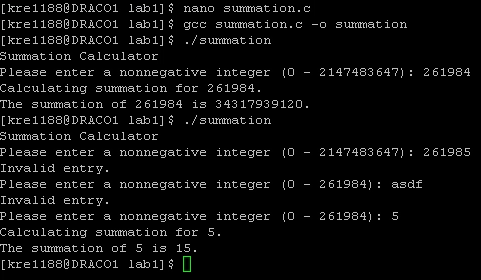
\includegraphics{screenshot.png}    
\end{center}

The apparent limit of recursion from my testing on DRACO1 revealed an upper limit at $n=261,984$.
This is due to the stack limit, as higher values create a stack overflow resulting in a segmentation fault as the recursion depth gets higher.
An interative approach would not be limited by this, and would likely be able to calculate any sums up to limits of integer implementations.

\end{document}